%
% File acl2014.tex
%
% Contact: koller@ling.uni-potsdam.de, yusuke@nii.ac.jp
%%
%% Based on the style files for ACL-2013, which were, in turn,
%% Based on the style files for ACL-2012, which were, in turn,
%% based on the style files for ACL-2011, which were, in turn, 
%% based on the style files for ACL-2010, which were, in turn, 
%% based on the style files for ACL-IJCNLP-2009, which were, in turn,
%% based on the style files for EACL-2009 and IJCNLP-2008...
%% Based on the style files for EACL 2006 by 
%%e.agirre@ehu.es or Sergi.Balari@uab.es
%% and that of ACL 08 by Joakim Nivre and Noah Smith

\documentclass[11pt]{article}
\usepackage{acl2014}
\usepackage{times}
\usepackage{url}
\usepackage{latexsym}
\usepackage{amsmath}

\usepackage[usenames,dvipsnames,svgnames,table]{xcolor}
\usepackage{soul}

\usepackage{algorithm}
\usepackage[noend]{algpseudocode}
\usepackage{graphicx}
\usepackage{caption}
\usepackage{subcaption}

\usepackage{tikz-dependency}


\newcommand{\Note}[1]{}
\renewcommand{\Note}[1]{\hl{[#1]}}  % comment out this definition to suppress all Notes                                                                                
\newcommand{\TODO}[1]{\Note{TODO: #1}}
\newcommand{\NoteSigned}[3]{{\sethlcolor{#2}\Note{#1: #3}}}
\newcommand{\NoteJE}[1]{\NoteSigned{JE}{LightBlue}{#1}}
\newcommand{\NoteJH}[1]{\NoteSigned{JH}{YellowGreen}{#1}}






\title{Deriving Multi-headed Planar Dependency Parses from Link Grammar Parses}

\author{Juneki Hong and Jason Eisner\\
  Department of Computer Science \\
  Johns Hopkins University \\
  Baltimore, MD 21218, USA \\ 
  {\tt \{juneki,jason\}@cs.jhu.edu} \\
}

\date{}

\begin{document}
\maketitle

\begin{abstract}

% Copied from the google doc
There has been recent theoretical work on multi-headed versions of dependency grammar (cite). Such formalisms can be more syntactically and semantically expressive. However, there aren't any corpora at present (check this) except for Buch-Kromann's work on Danish (cite), so it is hard to investigate the benefit of such parsers or to work on making them faster or more accurate. To fill this gap, we observe that link grammar produces parses that are similar to multi-headed planar dependency parses except that the links are undirected. We use Integer Linear Programming to assign consistent directions to the links in a corpus of NNN parses produced by the Link Grammar Parser, which has broad-coverage hand-written grammars of English, Russian, and more. (what statistics does it use?). We find that such directions can indeed be consistently assigned in a way that yields valid multi-headed dependency parses. The resulting parses in English appear linguistically plausible, although they are not in general consistent with CoNLL-style parses of the same sentences; we discuss the differences. We also report ...

\end{abstract}



\section{Introduction}


Dependency parsing is the task of mapping a sentence to a projective (not always projective?) directed acyclic tree. Link parsing in contrast produces a multiheaded planar graph with undirected edges, where every edge has a label describing the relationship between two constituents in a parse. In this paper we explore whether these relationships include dependencies. To determine the directional dependencies within the link edge labels we will use integer linear programming, encoding the problem in the Zimpl little language \cite{Koch2004}. It turns out that the link parses roughly only match half of the conll dependency corpus. However this is because \TODO{}. 

%Despite this, the link parses offer additional links in addition to dependencies...




\section{Link Grammars}

Link grammars describe the links, or relationships between constituents in a parse \cite{SleatorTemperly91}. 


We ran the link parser on the english bnews corpus sentences \footnote{We ignored the link parses that the link parser could not find suitable attachments and returned a disconnected graph. This happened for roughly NNN\% of the corpus.}

The link grammar on which the link-parser makes its linking decisions based on a set of handwritten dictionaries. Instead of going through these dictionaries, we learned the link grammar using an ILP. This approach allows us to analyze any link grammar dictionary other than English.



\section{Integer Linear Programming}

We formulated the ILP to assign directional dependencies to a link grammar parse such that it is a connected DAG, with all of the nodes reachable from the root.

The ILP chooses whether to set a link type to be assigned left, right, or both. For this, two label\_direction variables were made for each link type that appears in the parses, corresponding to whether all of the $l$ link edges were to be set to go left, right, or both. Because we assign a directionality to every link type, at least one of these variables must be set to true.

For example, setting the variables $$l_{LEFT} = TRUE, l_{RIGHT} = FALSE$$ would mean that the directional dependency of all links with label $l$ would be set to $LEFT$. If both variables were set to true, then the link type is allowed to go in either direction. Our ILP objective is to minimize the number of label\_direction variables set to true, while satisfying the other constraints.

\TODO{cite model minimization papers}


\subsection{Slack Hierarchy}

We introduced slack on the directional dependency variable tokens such that link types were allowed to deviate from the majority up to (1\% ?) of the time before the ILP would assign both directional dependency variables to true. This addressed noise in the link parser's label assignments, while still allowing for the possibility that both directions could still be assigned.

\TODO{} We also introduced slack on the link types such that link types with the same coarse grained label would try and align the same way as the majority in the group, where the preceding capital letters of the link type denote the coarse grained label, while the subscript letters denote further information. This slack places a prior on rare or never-before seen link types to be assigned in the same way as other similar link types.

This slack hierarchy gave the ILP the flexibility to handle noise and novel link types while still trying to learn the overall link grammar.


\begin{equation}
  count_{L, \textsc{left}} = \sum_{a \in \textsc{ARCS}_L} left_a
\end{equation}
\begin{equation}
  count_{L, \textsc{left}} = \textsc{M} \cdot \textsc{allowed}_{L,\textsc{left}} + \textsc{slack}_{L}
\end{equation}
Where $L \in \textsc{LABELS}$, and $\textsc{M}$ is the size of the corpus.
The objective is:
\begin{equation}
  \min \sum_{L \in \textsc{LABELS} \atop \textsc{DIR} \in \{left, right\}} (\textsc{allowed}_{L,\textsc{DIR}}) \atop + \textsc{COST}(L) * \sum_L \textsc{slack}_L
\end{equation}
\begin{equation}
  \textsc{COST}(L) = \frac{100}{(\textsc{count}_{L,\textsc{left}} + \textsc{count}_{L,\textsc{right}})}
\end{equation}


\begin{algorithm}
\caption{ILP Encoding}\label{ILP}
\begin{algorithmic}[1]
%\Procedure{MyProcedure}{}

\State $\text{min} \sum_{l \in labels} allowed_L(l) + allowed_R(l)$
\State $\text{subject to}$
\State $\text{Acyclicity}$
\State $\text{All nodes reachable from the root.}$

%\EndProcedure
\end{algorithmic}
\end{algorithm}



\subsection{Stability of Results}
We tested to see how the solution changed over increasing numbers of processed sentences. 
Taking the solution to the largest run as the answer key, we measured how much the previous runs deviated from it. We measured the precision of whether the assignments in the smaller runs matched the assignments of the largest run, and we measured the recall of whether the assignments in the largest run could be found in the smaller runs. 

\begin{figure}[ht!]
  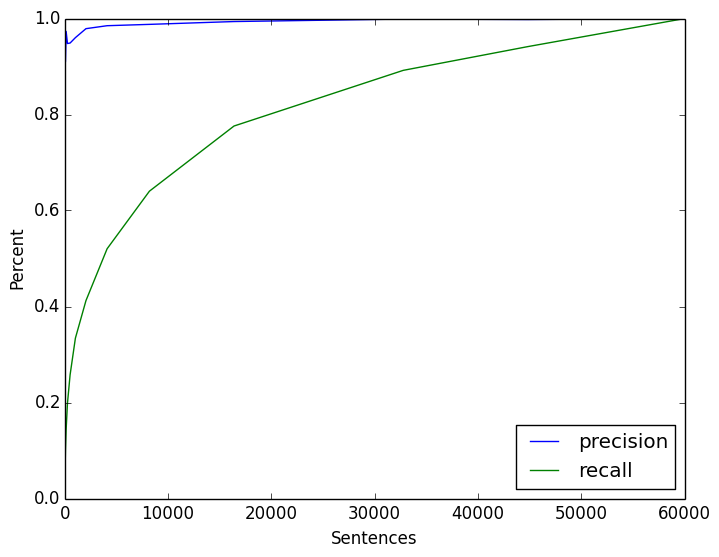
\includegraphics[width=\linewidth, keepaspectratio=true]{figure/precision_recall.png}
  \caption{Precision and Recall of different runs on English}
\end{figure}

In the end, the precision values converged to 100\% while the recall values continued to grow throughout our data. This indicates that the solutions of the previous runs were consistent with the largest run. However as the data grew, we would continue to encounter novel link types.



\section{Other languages}




\section{Link Corpus}


Compared to the original conll data, the link parses match about half the conll arcs in location and directionality. The mismatches in the other half can be accounted for in the following ways.

\subsection{Blanks}
Whenever the link parser failed to recognize a word from its dictionary, it would skip it and fail to attach any links. This accounts for about 10\% of the mismatches.

\subsection{Directional Mismatches}
In about 25\% of the cases, the conll arc's corresponding link would be assigned the opposite direction.


\section{Discussion}





\begin{figure*}[ht!]
  \centering
  \begin{subfigure}[b]{0.3233\textwidth}
	\begin{dependency}
		\begin{deptext}
			{\scriptsize PR} \& {\scriptsize VB} \& {\scriptsize RB} \& {\scriptsize VB} \& {\scriptsize .} \\
			it \& did \& n't \& work \& . \\
			- \& v-d \& - \& v \& - \\
		\end{deptext}
		\deproot[edge above, edge style = {blue, dotted}]{2}{\small ROOT}
		\depedge[edge below, edge style = {red, ultra thick}]{1}{2}{Ss}
		\depedge[edge above, edge style = {blue, thick}]{2}{1}{\small SBJ}
		\depedge[edge below, edge style = {red, thick}]{2}{3}{N}
		\depedge[edge above, edge style = {blue, thick}]{2}{3}{\small VMOD}
		\depedge[edge below, edge style = {red, thick}]{2}{4}{I*d}
		\depedge[edge above, edge style = {blue, thick}]{2}{4}{\small VC}
		\depedge[edge above, edge style = {blue, dotted}]{2}{5}{\small P}
		\deproot[edge below, edge style = {red, dotted}]{1}{Wd}
		\deproot[edge below, edge style = {orange, ultra thick}]{4}{WV}
		\deproot[edge below, edge style = {red, dotted}]{5}{Xp}
	\end{dependency}
\end{subfigure}
\begin{subfigure}[b]{0.3233\textwidth}
	\begin{dependency}
		\begin{deptext}
			{\scriptsize DT} \& {\scriptsize NN} \& {\scriptsize VB} \& {\scriptsize JJ} \& {\scriptsize .} \\
			the \& reason \& is \& simple \& . \\
			- \& n \& v \& a \& - \\
		\end{deptext}
		\deproot[edge below, edge style = {red, thick}]{3}{WV}
		\deproot[edge above, edge style = {blue, thick}]{3}{\small ROOT}
		\depedge[edge below, edge style = {red, thick}]{3}{2}{Ss*t}
		\depedge[edge above, edge style = {blue, thick}]{3}{2}{\small SBJ}
		\depedge[edge below, edge style = {red, thick}]{3}{4}{Paf}
		\depedge[edge above, edge style = {blue, thick}]{3}{4}{\small VMOD}
		\depedge[edge above, edge style = {blue, dotted}]{3}{5}{\small P}
		\depedge[edge below, edge style = {red, thick}]{2}{1}{D*u}
		\depedge[edge above, edge style = {blue, thick}]{2}{1}{\small NMOD}
		\deproot[edge below, edge style = {orange, ultra thick}]{2}{Wd}
		\deproot[edge below, edge style = {red, dotted}]{5}{Xp}
	\end{dependency}
\end{subfigure}
\begin{subfigure}[b]{0.3233\textwidth}
	\begin{dependency}
		\begin{deptext}
			{\scriptsize DT} \& {\scriptsize NN} \& {\scriptsize VB} \& {\scriptsize RB} \& {\scriptsize .} \\
			the \& judge \& wrote \& again \& . \\
			- \& n \& v-d \& - \& - \\
		\end{deptext}
		\deproot[edge below, edge style = {red, thick}]{3}{WV}
		\deproot[edge above, edge style = {blue, thick}]{3}{\small ROOT}
		\depedge[edge below, edge style = {red, thick}]{3}{2}{Ss}
		\depedge[edge above, edge style = {blue, thick}]{3}{2}{\small SBJ}
		\depedge[edge below, edge style = {red, thick}]{3}{4}{MVa}
		\depedge[edge above, edge style = {blue, thick}]{3}{4}{\small ADV}
		\depedge[edge above, edge style = {blue, dotted}]{3}{5}{\small P}
		\depedge[edge below, edge style = {red, thick}]{2}{1}{Ds}
		\depedge[edge above, edge style = {blue, thick}]{2}{1}{\small NMOD}
		\deproot[edge below, edge style = {orange, ultra thick}]{2}{Wd}
		\deproot[edge below, edge style = {red, dotted}]{5}{Xp}
	\end{dependency}
\end{subfigure}


  \caption{Example Sentences}
\end{figure*}



\section{Related Work}





\bibliographystyle{acl2014}
\bibliography{LinksToDAG}

\end{document}
